\section{Demonstração matemática}

Seja $g(t_1,t_2)$ uma função definida em todo o domínio $\mathcal{R}^2$ 
e $G(f_1,f_2)$ a sua respectiva transformada de Fourier.

\subsection{Inclinação bidimensional}
Para a propriedade de inclinação bidimensional, a função se molda de forma que
\begin{equation*}
    g(t_1 - \alpha t_2, t_2),
\end{equation*}

\noindent
onde $\alpha \in \mathcal{R}$  é o ângulo de inclinação no plano $(t_1,t_2)$.

Pela definição da transformada de Fourier bidimensional, temos que

\begin{equation*}
    G(f_1,f_2) = \int_{-\infty}^{+\infty} \int_{-\infty}^{+\infty} {g(t_1,t_2)e^{-j2\pi (f_1t_1+f_2t_2)}}dt_1dt_2,
\end{equation*}

\noindent
e para $g(t_1 - \alpha t_2, t_2)$

\begin{equation*}
    G(f_1',f_2') = \int_{-\infty}^{+\infty} \int_{-\infty}^{+\infty} {g(t_1 - \alpha t_2,t_2)e^{-j2\pi (f_1t_1+f_2t_2)}}dt_1dt_2.
\end{equation*}

Aplicando uma mudança de variáveis em $g(t_1 - \alpha t_2, t_2)$, podemos definir as variáveis de substituição


\begin{alignat}{4}
    v & = t_1 - \alpha t_2 &\quad& \Longrightarrow &\quad& t_1 = v + \alpha u, \\
    u & = t_2               &\quad& \Longrightarrow &\quad& t_2 = u.
\end{alignat}


% \begin{itemize}
%     \item $v = t_1 - \alpha t_2$ 
%     \item $u = t_2$
% \end{itemize}

Aplicando o jacobiano dessa transformação, obtemos
\[
J = 
\begin{vmatrix}
\frac{\partial t_1}{\partial v} & \frac{\partial t_1}{\partial u} \\
\frac{\partial t_2}{\partial v} & \frac{\partial t_2}{\partial u}
\end{vmatrix}
=
\begin{vmatrix}
1 & \alpha \\
0 & 1
\end{vmatrix}
= 1.
\]

Dado os limites iniciais $(-\infty,+\infty)$ de $t_1$ e $t_2$ as novas variáveis permanecerão com os mesmos limites de integração, obtendo assim


\begin{equation*}
    G(f_1',f_2') = \int_{-\infty}^{+\infty} \int_{-\infty}^{+\infty} {g(v,u)e^{-j2\pi (f_1(v +\alpha u)+f_2u)}}dvdtu,
\end{equation*}

\noindent
a partir do integrando obtido, podemos fatorar o conteúdo da exponencial em $-j2\pi(vf_1 + u(\alpha f_1 + f_2))$. Onde rearranjando obtemos

\begin{equation*}
    G(f_1',f_2') = \int_{-\infty}^{ +\infty} \int_{-\infty}^{+\infty} {g(v,u)e^{-j2\pi(vf_1 + uf_2)}e^{-j2\pi(u(f_1\alpha))}}dvdtu,
\end{equation*}

\noindent
o que resulta em
\begin{equation*}
      G(f_1',f_2') =\mathcal{F}\{g(v, u)e^{-j2\pi(u(f_1\alpha))}\}= G(f_1, \alpha f_1 + f_2).
\end{equation*}


\subsection{Rotação bidimensional}

Para a propriedade de rotação bidimensional, a função se molda para ser:

\begin{equation*}
    g(t_1',t_2'),
\end{equation*}

\noindent
onde

\[
\begin{bmatrix}
t_1' \\
t_2'
\end{bmatrix}
=
\begin{bmatrix}
\cos(\theta) & -\sin(\theta) \\
\sin(\theta) & \cos(\theta)
\end{bmatrix}
\begin{bmatrix}
t_1 \\
t_2
\end{bmatrix},
\]

\noindent
dessa forma

\begin{align}
    t_1 &= \cos\theta \cdot t_1' + \sin\theta \cdot t_2', \\
    t_2 &= -\sin\theta \cdot t_1' + \cos\theta \cdot t_2'.
\end{align}

Aplicando o jacobiano dessa transformação, obtemos:
\[
J = 
\begin{vmatrix}
\frac{\partial t_1}{\partial t_1'} & \frac{\partial t_1}{\partial t_2'} \\
\frac{\partial t_2}{\partial t_1'} & \frac{\partial t_2}{\partial t_2'}
\end{vmatrix}
=
\begin{vmatrix}
\cos\theta & \sin\theta \\
-\sin\theta & \cos\theta
\end{vmatrix}
= 1
\]


\begin{equation*}
    G(f_1',f_2') = \int_{-\infty}^{+\infty} \int_{-\infty}^{+\infty} {g(t_1',t_2')e^{-j2\pi (f_1(cos\theta \cdot t_1' + \sin\theta \cdot t_2')+f_2(-\sin\theta \cdot t_1' + cos\theta \cdot t_2')}}dt_1dt_2 
\end{equation*}

\noindent
onde fatorando o termo da exponencial em função de $t_1'$ e $t_2'$, obtemos

\begin{equation*}
    t_1'(f_1\cos\theta - f_2\sin\theta) + t_2'(f_1\sin\theta + f_2\cos\theta)
\end{equation*}

\noindent
o que resulta em

\begin{align}
\begin{split}
  G(f_1',f_2') &= G(f_1\cos\theta - f_2\sin\theta, f_1\sin\theta + f_2\cos\theta) \\
  &= \mathcal{F}\{g(t_1', t_2')e^{j2\pi t_1'f_2\sin\theta}e^{-j2\pi t_2'f_1\sin\theta}\}.
\end{split}
\end{align}


\section{Aplicação computacional}

Para a reprodução dos dados, foi usada a linguagem computacional \textbf{Python}, muito utilizada para processamento de imagens e tratamento de dados.

\subsection{Inclinação bidimensional}

Foi criada uma função \textit{shear\_image} para gerar a inclinação, que é dada abaixo:

\begin{lstlisting}
    def shear_image(img, a = 0, b = 0): # a: inclinação na horizontal, b: inclinação na vertical

    transformada = np.zeros_like(img)

    c = img.shape[0] // 2  # centro da imagem

    for x in range(img.shape[0]):
        for y in range(img.shape[1]):
            # Coordenadas centralizadas
            x_c = x - c
            y_c = y - c
            # Aplica inclinação centralizada
            x_src = int(round(x_c - a * y_c)) + c
            y_src = int(round(y_c - b * x_c)) + c
            if 0 <= x_src < img.shape[0] and 0 <= y_src < img.shape[1]:
                transformada[x, y] = img[x_src, y_src]
            else:
                transformada[x, y] = 0  # fora da imagem
    return transformada
\end{lstlisting}

\begin{figure}[H]
    \centering
    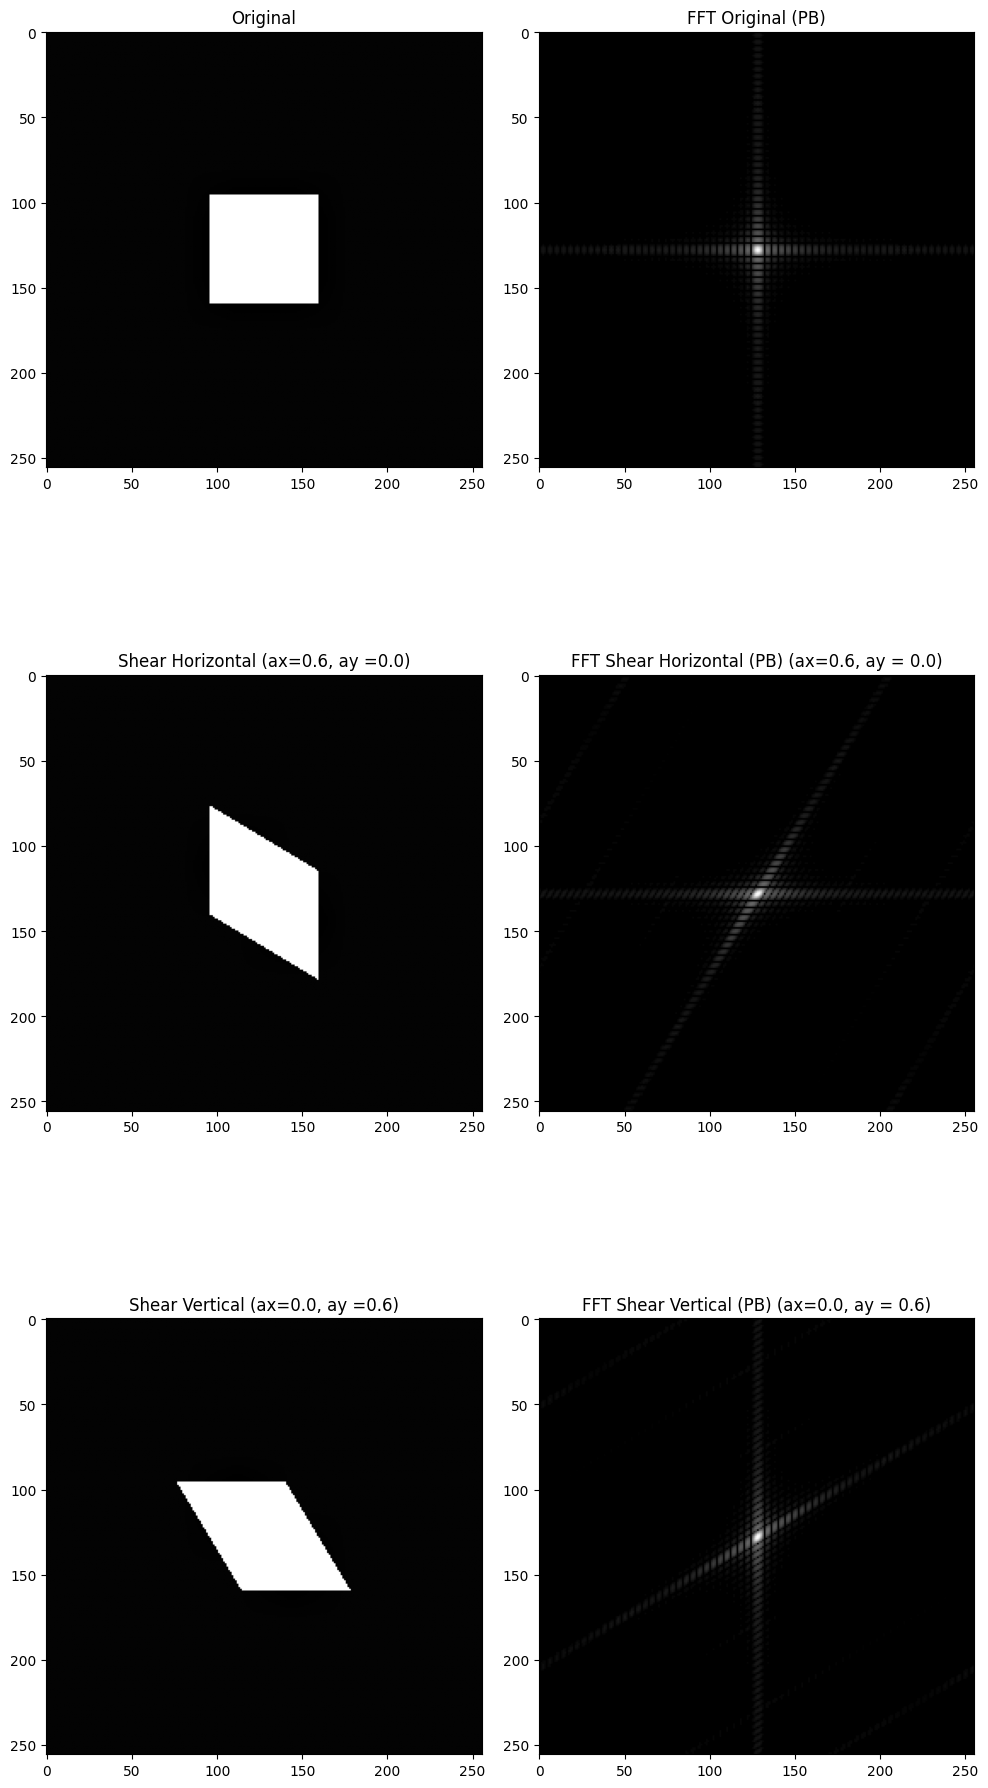
\includegraphics[width=0.75\linewidth]{figure/shear.png}
    \caption{Gráficos das figuras inclinadas e suas respectivas FFT's}
    \label{fig:placeholder}
\end{figure}


É possível notar que o efeito da inclinação também é observável na transformada de Fourier bidimensional. Como demonstrado matematicamente, a inclinação em $x$ na função inicial, gera uma inclinação em $y$ na sua transformada de Fourier. 

Por fim, é observável o espalhamento no espectro de frequência da imagem, causado pelo fato de estarmos tratando de um sinal discreto (pixels).

\subsection{Rotação bidimensional}
Foi criada uma função \textit{rotate\_image} para gerar a rotação, que é dada abaixo:

\begin{lstlisting}
def rotate_image(image, theta):
    # Pega as dimensões da imagem
    (h, w) = image.shape[:2]
    center = (w // 2, h // 2)
    rotated = np.zeros_like(image)

    # Cria grid de coordenadas de destino
    y_indices, x_indices = np.indices((h, w))
    x_c = x_indices - center[0]
    y_c = y_indices - center[1]

    # Aplica a rotação inversa para encontrar as coordenadas de origem
    cos_t = np.cos(np.radians(theta))
    sin_t = np.sin(np.radians(theta))
    x_src = cos_t * x_c + sin_t * y_c + center[0]
    y_src = -sin_t * x_c + cos_t * y_c + center[1]

    # Interpola os valores da imagem original nas novas coordenadas
    rotated = map_coordinates(image, [y_src.ravel(), x_src.ravel()], order=1, mode='constant', cval=0)
    rotated = rotated.reshape((h, w))
    return rotated
\end{lstlisting}

A interpolação é feita para remover os "buracos" de pixel causadas pelos arrendondamentos da rotação.

\begin{figure}[H]
    \centering
    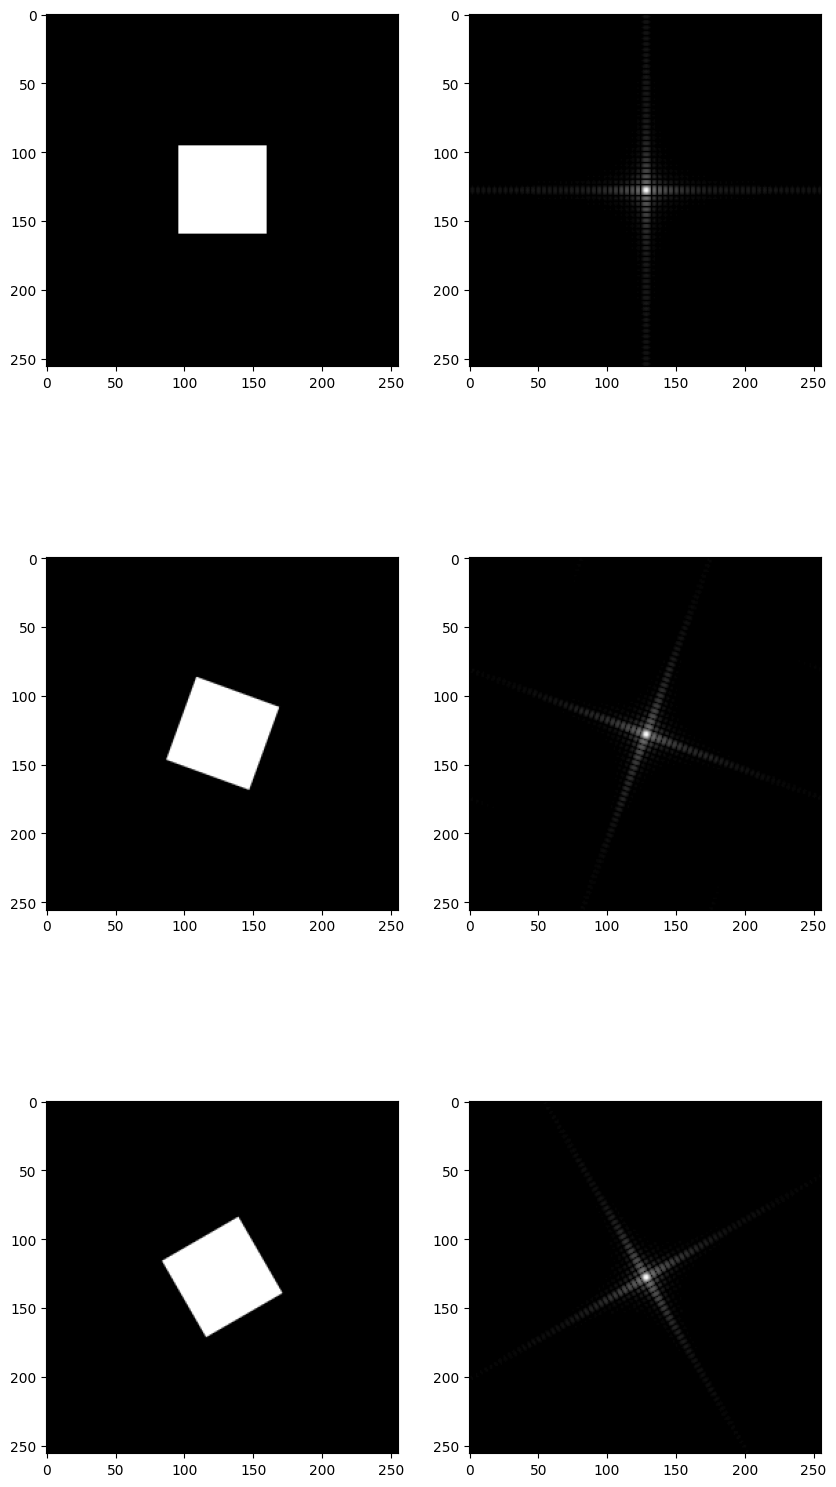
\includegraphics[width=0.75\linewidth]{figure/rotate.png}
    \caption{Gráficos das figuras rotacionadas e suas respectivas fft´s}
    \label{fig:placeholder}
\end{figure}

Da mesma forma que demonstrado antes, a rotação da imagem original gera uma mesma rotação (variação de parâmetros) na sua transformada de Fourier.